% !TEX encoding = UTF-8
% !TEX TS-program = pdflatex
% !TEX root = ../tesi.tex

%**************************************************************
\chapter{Processi e metodologie}
\label{cap:processi-metodologie}
%**************************************************************

In questo capitolo verrà fornita una descrizione dei metodi e dei processi messi in atto durante il tirocinio e in particolare riguardo: la metodologia agile, la programmazione funzionale, la gestione del progetto in locale e l'organizzazione del lavoro.

%**************************************************************
\section{Metodologia Agile}
Per lo sviluppo del prodotto è stato deciso di applicare una metodologia agile in modo da reagire velocemente a possibili problemi e cambiamenti dei requisiti così da migliorare e velocizzare la realizzazione dell'applicativo. L'azienda ha deciso di utilizzare una metodologia agile simile a \gls{scrumg}. Infatti applicare nella sua interezza il metodo \emph{SCRUM} sarebbe stato impossibile dato il ristretto numero di sviluppatori nel team di sviluppo e il limitato periodo riservato alla codifica. \\
Le caratteristiche principali della metodologia agile applicata per la realizzazione di questo progetto sono le seguenti:
\begin{itemize}
	\item \textbf{Modello incrementale}: vengono realizzati rilasci multipli e successivi che aiutano a definire più chiaramente i requisiti più importanti dato che essi verranno implementati per primi. Ogni rilascio corrisponde ad una parte funzionante di applicazione;
	
	\item \textbf{Modello iterativo}: un modello iterativo ha la caratteristica di avere una maggior capacità di adattamento in seguito a problemi di implementazione e cambiamenti nei requisiti;
	
	\item \textbf{Organizzazione in sprint di sviluppo}: il periodo di codifica viene suddiviso in sprint di sviluppo, data la breve durata del tirocinio curriculare essi avranno una durata di circa 4-5 giorni.
\end{itemize}
\noindent
Gli elementi che caratterizzano la metodologia agile utilizzata sono:
\begin{itemize}
	\item \textbf{Product backlog}: documento molto importante che contiene i requisiti e le funzionalità del prodotto definiti mediante le \emph{User Stories} ordinate per priorità (\emph{Business value});
	
	\item \textbf{Sprint backlog}: rappresenta l'insieme delle User Stories da realizzare nello sprint;
	
	\item \textbf{Increment}: insieme di tutte le user stories che sono state completate dall'ultima release del software.
\end{itemize}
\noindent
La metodologia agile applicata presenta inoltre i seguenti eventi che sono stati ripetuti ogni settimana in corrispondenza di ogni sprint:
\begin{itemize}
	\item \textbf{Sprint Planning}: riunione tra i partecipanti del team di sviluppo dove vengono determinati quali user stories del product backlog verranno completate nello sprint;
	
	\item \textbf{Daily Stand-up}: breve riunione giornaliera dove ogni membro descrive velocemente i progressi dall'ultimo \emph{Daily Stand-up}, i problemi riscontrati e i suoi prossimi obiettivi, questo evento è stato, in molte occasioni, sostituito da una riunione telematica;
	
	\item \textbf{Sprint Review}: riunione dove viene mostrato il prodotto con tutte le modifiche completate durante lo sprint (\emph{increment});
	
	\item \textbf{Backlog refinement}: riunione per aggiungere, modificare o eliminare user stories dal \emph{product backlog};
	
	\item \textbf{Retrospective}: riunione finale dove vengono determinati i fattori positivi e negativi in modo da identificare le strategie migliori per ottenere un miglioramento continuo dei processi.
\end{itemize}
\noindent
%\begin{minipage}{\linewidth}
%	\makebox[\linewidth] {
%		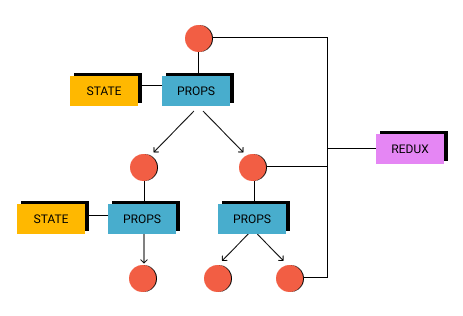
\includegraphics[scale=0.75]{./immagini/dataflow_react_redux.png}
%	}
%\end{minipage}

\section{Programmazione funzionale}
La programmazione funzionale è un paradigma di programmazione dichiarativa dove un programma è costituito dall'applicazione e dalla composizione di funzioni. In questo progetto si è utilizzata, dove possibile, la programmazione funzionale mediante le \gls{hofg} fornite da Kotlin. Questi strumenti sono molto utili perchè permettono di scrivere un codice più leggibile, conciso. Soprattutto hanno la caratteristica di evitare \gls{sideeffectsg}. Come definito dalla documentazione di Kotlin, le funzioni scritte nel linguaggio Kotlin sono considerate come \emph{first-class} quindi esse possono essere contenute in variabili e strutture dati, passate come argomento di altre funzioni e ritornate da altre \emph{Funzioni di ordine superiore}. Le \emph{higher-order functions} più usate nel progetto sono state:
\begin{itemize}
	\item \verb|map|: ritorna una nuova lista contenente i risultati ottenuti dalla funzione di trasformazione per ogni elemento della collezione originale;
	\item \verb|sortedWith|: ritorna una lista contenente tutti gli elementi della lista originale ordinati secondo un \verb|comparator| una funzione che impone una condizione tra gli elementi della lista;
	\item \verb|flatMap|: stesse funzionalità di \verb|map| ma può essere invocato su più di una lista e ritorna una collezione unica;
	\item \verb|groupBy|: raggruppa gli elementi di una lista ottenuta con i risultati della funzione \verb|keySelector| applicata ad ogni elemento della lista originale, ritorna una collezione di tipo: \verb|Map<K, V>|.
\end{itemize}
Oltre all'uso delle \emph{Funzioni di ordine superiore} il paradigma di programmazione funzionale è stato applicato anche all'architettura dell'applicazione infatti è stato utilizzato un'insieme di funzioni dichiarative rispetto ad una gerarchia di classi ed una sequenza di operazioni imperative che cambiano lo stato del programma.

\section{Versionamento della soluzione}
\subsection{Git}
Git è un \gls{vcsg} distribuito che permette di tenere traccia delle modifiche in un prodotto software e di organizzarne la codifica. 

\subsubsection*{Feature-branch}
In questo tirocinio è stata usata la tecnica del feature-branch: ogni aggiunta di feature corrisponde all'apertura di un nuovo branch che deve essere poi approvato previa verifica prima di essere unito al branch \verb|master| mediante una \emph{pull request}.

\subsection{Gitlab}
Gitlab è uno strumento web che permette di implementare un DevOps lifecycle che fornisce una gestione di repository git, un \gls{itsg} e altri strumenti quali la \emph{Continuous integration} e \emph{Continuous deployement}. Per lo sviluppo di questo progetto mi è stato fornito l'accesso al server privato aziendale Gitlab.

\section{Ambiente di sviluppo locale}
\subsection{IntelliJ Idea}
IntelliJ IDEA Community Edition è una \gls{ideg} realizzata da JetBrains che fornisce funzionalità di supporto per lo sviluppo di molti linguaggi, specialmente Kotlin. Questa \emph{IDE} è stata vivamente consigliata dal mio tutor aziendale per lo sviluppo in Kotlin rispetto ad altri editor per molti vantaggi come l'autocompletamento, la possibilità di eseguire un refactoring automatico di funzioni e classi e un'interfaccia grafica per eseguire task di Gradle.
 
\subsection{Gradle}
Gradle è uno strumento di \gls{buildautomationg} per molti linguaggi tra cui Kotlin e Java. Gradle è stato usato per la gestione e l'installazione delle dipendenze del componente, il file di configurazione di Gradle è \verb|build.gradle.kts|, al suo interno sono definite le seguenti dipendenze:
\begin{itemize}
	\item \verb|stdlib-js|: insieme di classi e funzioni in kotlin che forniscono un entry-point per funzioni e oggetti Javascript;
	
	\item \verb|kotlin-react|: implementazione di kotlin della liberia React;
	
	\item \verb|react|: pacchetto npm della libreria React necessario per il funzionamento di \verb|kotlin-react|;
	
	\item \verb|kotlin-redux|: implementazione di kotlin della libreria Redux;
	
	\item \verb|kotlin-react-redux|: implementazione di kotlin della libreria React, Redux;
	
	\item \verb|kotlin-extensions|: libreria che fornisce dei \emph{wrapper} per oggetti JS e alcune funzione \emph{helper} per \verb|kotlin-react|;
	
	\item \verb|kotlinx-serialization-core|: libreria utilizzata per ottenere funzioni di parse per JSON;
	
	\item \verb|test-js|: libreria di test per Kotlin/js;
	
	\item \verb|kotlinx-coroutines-core|: libreria utilizzata per eseguire funzioni asincrone.
\end{itemize}
\noindent
Oltre alla gestione delle dipendenze Gradle offre delle task, utili per compilare ed eseguire l'applicativo. Nell'ambito del progetto ho utilizzato la task: \verb|runDevelopment| e come parametro della task: \verb|--continuous| in modo da eseguire automaticamente la compilazione del codice quando viene cambiato uno dei file sorgente; questo risulta molto utile quando si codifica un'interfaccia web dato che i cambiamenti vengono visualizzati automaticamente.

\subsection{Organizzazione del lavoro}
Per l'organizzazione del lavoro, in particolare per la gestione dei macro obiettivi di ogni sprint, ho utilizzato l'\emph{ITS} fornito da Gitlab che fornisce un'interfaccia \emph{Kanban} che permette di categorizzare in modo efficace le singole attività da realizzare. \\
Per quanto riguarda le riunioni telematiche è stato usato \emph{Google meet}.
























